\documentclass[frenchb]{beamer}
\usepackage{tabularx}
\usepackage[utf8]{inputenc}
\usepackage{babel}
\usepackage[T1]{fontenc}

\usecolortheme{whale}
\title{TX-TIPE Chariot}
\subtitle{Etude et optimisation du parcours d'un chariot :\\conception d'un algorithme de cheminement}
\date{P19\\15 Juillet 2019}
\institute{Lycée Pierre d'Ailly - Université de Technologie de Compiègne}
\author{Romain Maliach-Auguste}
\begin{document}
\frame{\titlepage}
  \begin{frame}
    \frametitle{Présentation du travail effectué}
	  \begin{itemize}
			 \item Implémentation des résultats mécaniques de mon binôme
			 \item Simplification du modèle de la grille et détermination d'une structure de données adaptée
			 \item Adaptation d'algorithmes connus et prouvés au problème
			 \item Implémentation et tests
	  \end{itemize}
  \end{frame}
  \begin{frame}
	  \frametitle{Résultats mécaniques de mon binôme}
		Durée minimale en virage:\[t_1 = \pi\sqrt{\frac{R_c(r+e)}{2lg}}\]
		où l est l'écart des roues, $R_c$ est le rayon de courbure, $r$ est le rayon des roues, $e$ la hauteur du colis (assimilé au centre de gravité).

		Durée minimale en ligne droite:
		\[t_2=2\sqrt{\frac{d}{fg}}\]
		où $d$ est la longueur du couloir et $f$ le coefficient de frottement.
	 
	  \begin{figure}
		  \centering
		  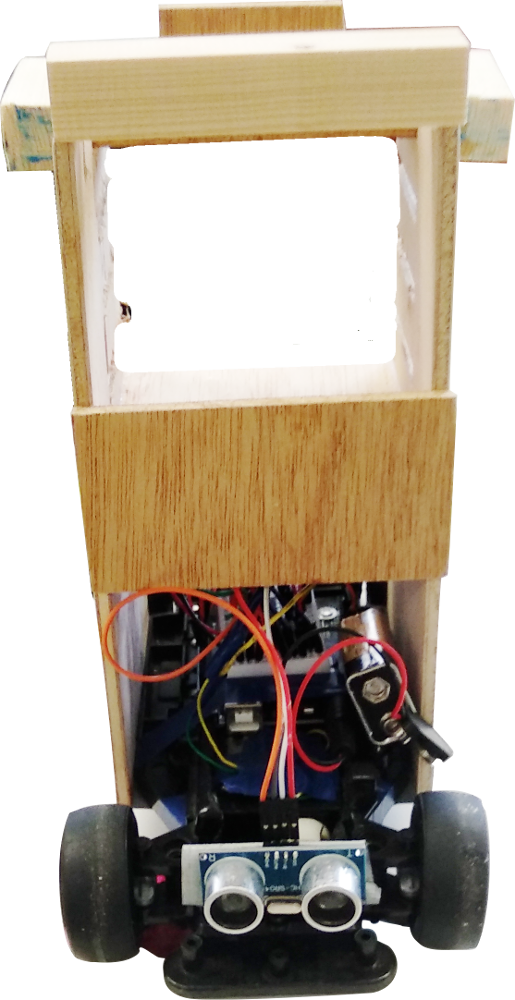
\includegraphics[height=2cm]{protoChariot.png}
		  \caption{Le modèle réduit utilisé pour nos tests}
	  \end{figure}
  \end{frame}
  \begin{frame}
	  \frametitle{Modèle de la grille}
  \end{frame}
\end{document}
